
\subsection{Beyond accuracy on downstream tasks}
When studying the impact of scaling, there are important aspects to consider beyond downstream task performance. In this section, we probe \chonk's fairness, alignment with human perception, robustness, reliability, and calibration. We find that favorable characteristics emerge when increasing model size. Additional analysis on perceptual similarity and feature attribution can be found in \cref{app:perceptual_similarity} and \cref{app:feature_attribution}.


\subsubsection{Fairness}\label{sect::fairness}
Machine learning models are susceptible to unintended bias. For example, they can amplify spurious correlations in the training data~\citep{hendricks2018women,caliskan2017semantics,zhao2017men,wang2020towards} and result in error disparities~\citep{zhao2017men,buolamwini2018gender,deuschel2020uncovering}. 
Here, we identify how scaling the model size can help mitigate such issues, by evaluating the bias of \chonk  and ViT-\{L, g, G, e\} ~\citep{zhai2022scaling,chen2022pali} using demographic parity (DP) as a measure of fairness~\citep{dwork2012fairness,zafar2017fairness}.

\begin{figure}[hbt!]
    \centering
    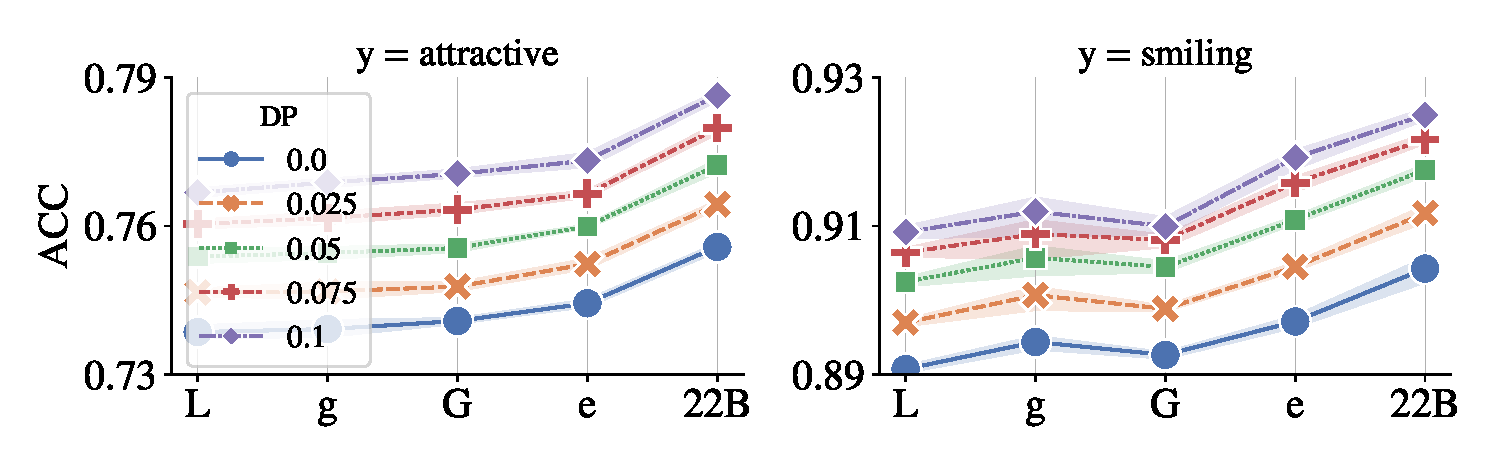
\includegraphics[width=0.7\columnwidth]{figs/fairness/perf_acc.v3.pdf}
    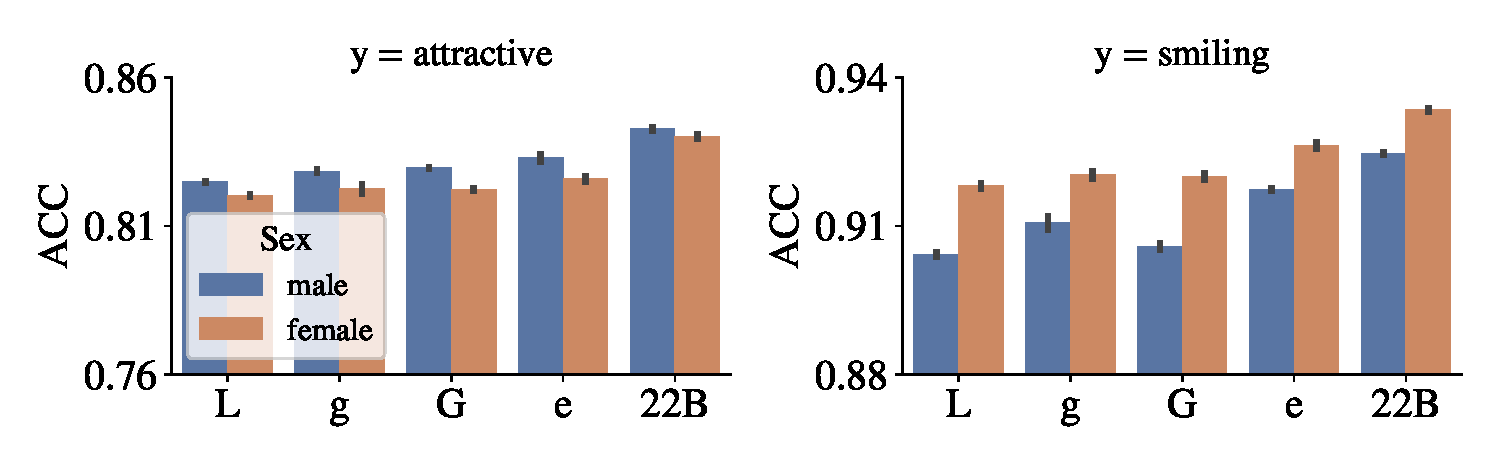
\includegraphics[width=0.7\columnwidth]{figs/fairness/all_benefit_acc_1.v3.pdf}
    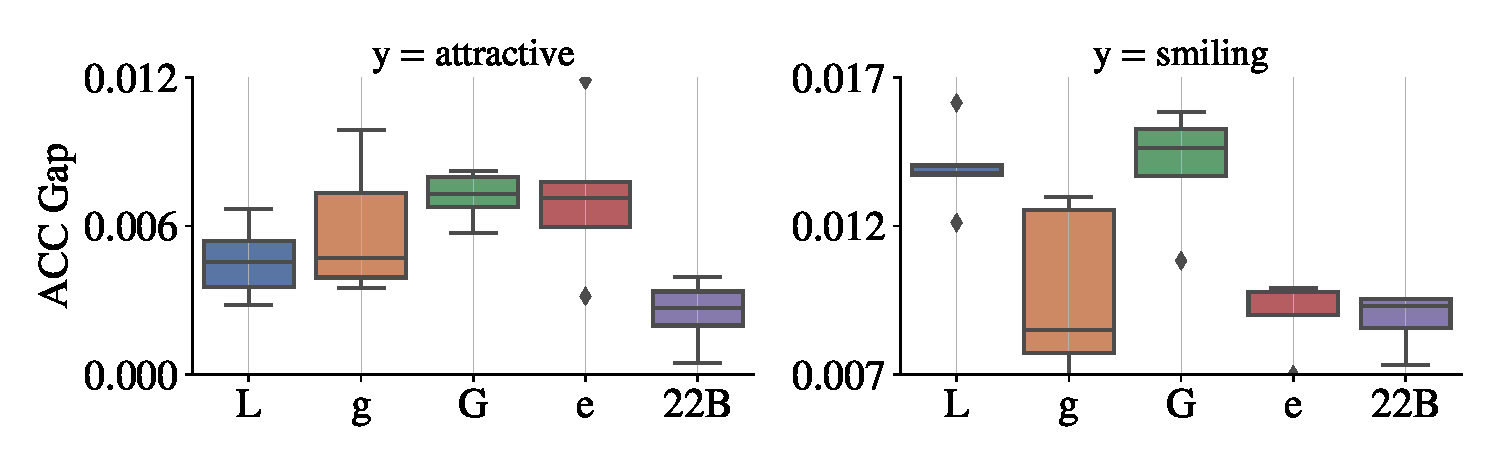
\includegraphics[width=0.7\columnwidth]{figs/fairness/parity_acc_1.v3.pdf}
    \vspace{-10pt}
    \caption{{\sc top:} Accuracy (ACC) for ViT variants \emph{after} debiasing for each DP level.  {\sc middle}: Accuracy for each subgroup in CelebA \emph{prior to} debiasing. {\sc bottom}:  $y$-axis is absolute difference in performance across the two subgroups: females and males. \chonk provides a more equitable performance, compared to smaller ViT architectures.}
    \label{fig:fairness:main}
    \vspace{-10pt}
\end{figure}

% Given a domain $\mathcal{X}$ (e.g. images) a total partitioning of $\mathcal{X}$ into subgroups $\mathcal{X}=\cup_k\mathcal{X}_k$ (e.g. based on gender or race), let $f:\mathcal{X}\to\{0, 1\}$ be a binary predictor. Then, demographic parity (DP) in $f$ with respect to $\{\mathcal{X}_k\}_k$ is defined as~\citep{dwork2012fairness,zafar2017fairness}: 
% \begin{equation}\label{eq:dp}
%     DP_f = \max_{k}\mathbb{E}[f(\textbf{x})|\textbf{x}\in\mathcal{X}_k] - \min_{k}\mathbb{E}[f(\textbf{x})|\textbf{x}\in\mathcal{X}_k].
% \end{equation}
% Extensions to the multiclass setting exist~\citep{alabdulmohsin2022}, but we focus on binary classification.


\paragraph{Experimental Setup.} We use CelebA~\citep{liu2015faceattributes} with binary gender as a sensitive attribute while the target is  ``attractive'' or ``smiling''. We emphasize that such experiments are carried out only to verify technical claims and shall by no means be interpreted as an endorsement of such vision-related tasks. We choose the latter attributes because they exhibit gender related bias as shown in \cref{fig:fairness:bias_original}.

We train a logistic regression classifier on top of the \chonk pretrained features for a total of $50$ epochs and batch size $256$, with a learning rate schedule of $0.01$ (first 25 epochs) and 0.001 (last 25 epochs).  After that, we debias using the randomized threshold optimizer (RTO) algorithm of~\citet{alabdulmohsin2021}, which was shown to be near-optimal and competitive with in-processing methods. %In RTO, we use 10K SGD steps and 1K full gradient steps, while keeping the other settings to their default values.

\paragraph{Results.}
We observe that scale by itself does not impact DP, c.f.\ \cref{fig:fairness:bias_original}. This is perhaps not surprising, as the model is trained to reconstruct a chosen target so the level of DP in accurate models is similar to that of the data itself.

However, scaling to \chonk offers benefits for fairness in other aspects. First, scale offers a more favorable tradeoff ---  performance improves with scale subject to any prescribed level of bias constraint.
This is consistent with earlier observations reported in the literature~\citep{alabdulmohsin2021}.  Second, all subgroups tend to benefit from the improvement in scale. Third, \chonk reduces disparities in performance across subgroups. 
\cref{fig:fairness:main} summarizes results for classification accuracy and \cref{app:fairness} for expected calibration error (ECE)~\citep{naeini2015obtaining,guo2017calibration} and OC-AUC~\citep{kivlichan2021measuring}.
%We use on three metrics: (1) classification accuracy (denoted ACC), (2) expected calibration error (ECE)~\citep{naeini2015obtaining,guo2017calibration}, and (3) Oracle Collaborative AUC (OC-AUC)~\citep{kivlichan2021measuring}.


\subsubsection{Human Alignment}
\label{subsec:error consistency}
%

How well do \chonk classification decisions align with human classification decisions? Using the {\tt model-vs-human} toolbox~\citep{geirhos2021partial}, we evaluate three \chonk models fine-tuned on ImageNet with different resolutions (224, 384, 560). Accross all toolbox metrics, \chonk is SOTA: \chonk-224 for highest OOD robustness (\cref{fig:model_vs_human_benchmark_a}), \chonk-384 for the closest alignment with human classification accuracies (\cref{fig:model_vs_human_benchmark_b}), and \chonk-560 for the largest error consistency (i.e.\ most human-like error patterns, \cref{fig:model_vs_human_benchmark_d}). The \chonk models have the highest ever recorded shape bias in vision models: while most models have a strong texture bias (approx.\ 20--30\% shape bias / 70--80\% texture bias)~\citep{geirhos2019imagenet}; humans are at 96\% shape / 4\% texture bias and \chonk-384 achieves a previously unseen 87\% shape bias / 13\% texture bias (\cref{fig:shape_bias}). Overall, \chonk measurably improves alignment to human visual object recognition.

\begin{figure}
    \centering
    \vspace{-5pt}
    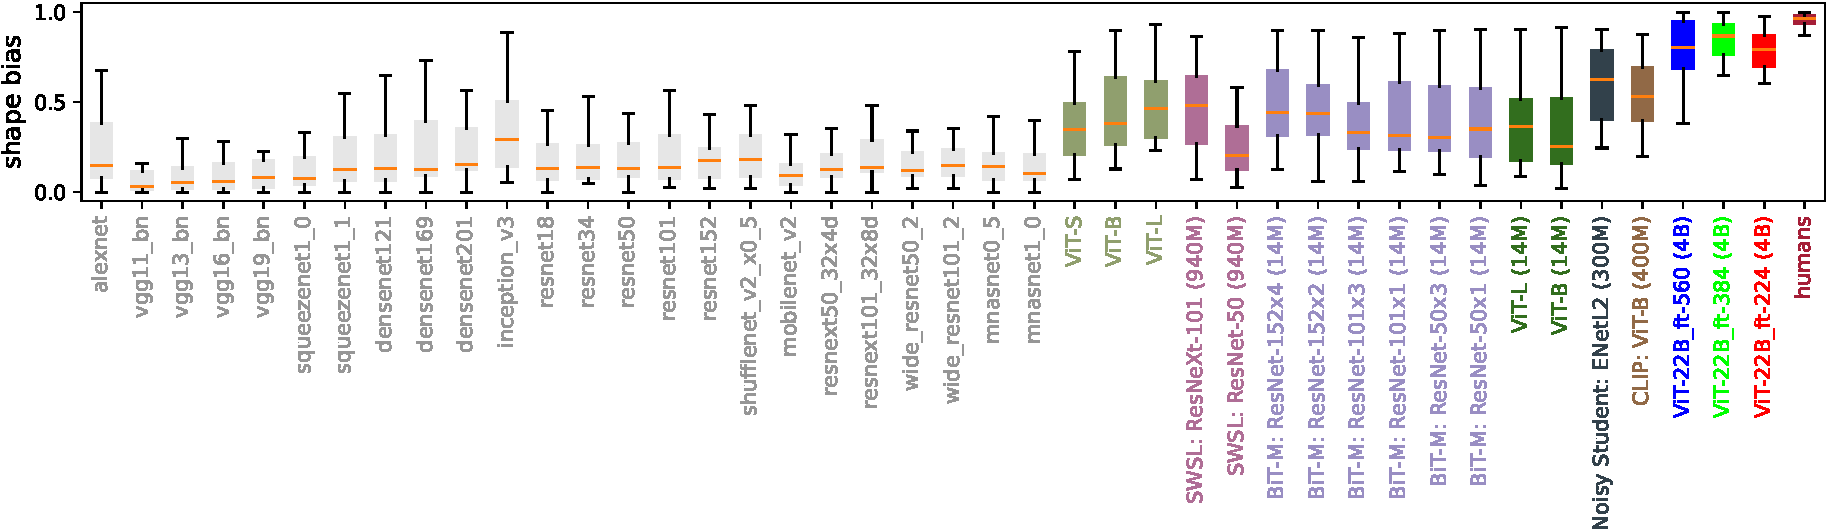
\includegraphics[width=\textwidth]{figs/human-alignment/cue-conflict_shape-bias_boxplot.pdf}
    \vspace{-0.8cm}
    \caption{Shape bias: many vision models have a low shape / high texture bias, whereas \chonk fine-tuned on ImageNet (\textcolor{red}{red}, \textcolor{green}{green}, \textcolor{blue}{blue} trained on 4B images as indicated by brackets after model names, unless trained on ImageNet only) have the highest shape bias recorded in a ML model to date, bringing them closer towards a human-like shape bias.}
    \label{fig:shape_bias}
\vspace{-10pt}
\end{figure}
%


\subsubsection{Plex - pretrained large model extensions}
\citet{tran2022plex} comprehensively evaluate the reliability of models through the lens of uncertainty, robustnes (see \cref{subsec:robustness_ood}) and adaptation (see \cref{sect::lit}).
% In this section, we focus on the first aspect of that benchmark. 
We focus here on the first aspect of that benchmark. 
To this end, we consider (1) the OOD robustness under
covariate shift with ImageNet-C~\citep{hendrycks2019benchmarking}, which we evaluate not only with the accuracy but also uncertainty metrics measuring the calibration (NLL, ECE) and the selective prediction~\citep{el2010foundations} (OC-AUC, see \cref{sect::fairness}), and (2) open-set recognition---also known as OOD detection~\citep{fort2021exploring}, which we evaluate via the AUROC and AUPRC, with Places365 as the OOD dataset~\citep{hendrycks2019scaling}; for more details, see \cref{app:plex}.

% , selective prediction~\citep{el2010foundations} 
% and label uncertainty~\citep{dusenberry2020analyzing}.

In \cref{tab:plex}, we report the performance of ViT-L and ViT-22B (both with resolution 384) fine-tuned on ImageNet. 
To put in perspective the strong gains of ViT-22B, we also show Plex-L, a ViT-L equipped with the two components advocated by \citet{tran2022plex}, viz, efficient-ensemble~\citep{wen2019batchensemble} and heteroscedastic layers~\citep{collier2021correlated}.
% to better capture model and data uncertainty respectively (Plex-L). 
We discuss the challenges and the results of the usage of those components at the 22B scale (Plex-22B) in \cref{app:plex}.

% \begin{table}[t]
%     \caption{Placeholder for PLEX~\citep{tran2022plex} results.}
% \centering
% \small
%   \setlength{\tabcolsep}{4pt}
%   \resizebox{\columnwidth}{!}{%
%     \begin{tabular}{@{} l c c c c c @{}}
%       \toprule
% 	    Evaluations      & IN-C & OOD det. & Sel.~Pred. & Lab.~Unc. \\
%       \midrule
%       ViT-L~\citep{tran2022plex} &  &  &  &  & \\
%       \chonk (Ours) &  &  &  &  &  \\
%       PLEX-L~\citep{tran2022plex} &  &  &  &  & \\
%       PLEX-22B (Ours) &  &  &  &  &  \\
%       \bottomrule
%  \end{tabular}
%  }
%     \label{tab:plex}
% \end{table}

\begin{table}[t]
    \caption{ViT-22B evaluated on some representative metrics from the Plex reliability benchmark~\citep{tran2022plex}$^*$.}
\centering
  \setlength{\tabcolsep}{4pt}
  \resizebox{.6\textwidth}{!}{%
    \begin{tabular}{@{} l @{} c ccc c ccc @{}}
      \toprule
       && \multicolumn{4}{c}{IN-C (mean over shifts)} && \multicolumn{2}{c}{IN vs.~Places365} \\
      % && \multicolumn{3}{c}{Linear~\citet{strudel2021segmenter}} && \multicolumn{3}{c}{UperNet~\citet{xiao2018unified}} \\
\cmidrule{3-6}\cmidrule{8-9}
	      Metrics && ACC $\uparrow$ & NLL $\downarrow$ & ECE $\downarrow$ & OC-AUC $\uparrow$ && AUROC $\uparrow$ & AUPRC $\uparrow$ \\
      \midrule
      ViT-L/32$^*$ &&  70.1 & 1.28 &  0.05 & 0.91 && 0.83 &  0.96 \\
      Plex-L/32$^*$ &&  71.3 & 1.21 & 0.02 &  0.91 && 0.83 &  0.97 \\
      ViT-22B && \textbf{83.7} & \textbf{0.63} &  \textbf{0.01} & \textbf{0.97} && \textbf{0.88} &  \textbf{0.98}  \\
      \bottomrule
 \end{tabular}}
    \label{tab:plex}
% \vspace{-10pt}
\end{table}


\subsubsection{Calibration}
\label{subsec:calibration}
Along with the robustness of \cref{subsec:robustness_ood}, it is also natural to wonder how the calibration property of ViT evolves as the scale increases. To this end, we focus on the study of \citet{minderer2021revisiting} that we extend with \chonk.

In \cref{fig:calibration}, we consider \chonk fine-tuned on ImageNet (resolution 384) and report the error (i.e., one minus accuracy) versus the calibration, as measured by the expected calibration error (ECE)~\citep{naeini2015obtaining,guo2017calibration}.
We see how \chonk remarkably improves the tradeoff between accuracy and calibration. The conclusion holds both without (left) and with (right) a temperature-scaling of the logits that was observed to better capture the calibration trends across model families~\citep{minderer2021revisiting}. More details can be found in \cref{app:calibration}.

\begin{figure}[tbp]
    \centering
    \subfigure[Unscaled]{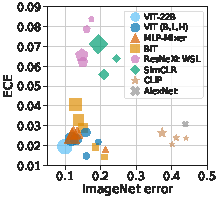
\includegraphics[width=0.35\textwidth]{figs/calibration_plex/vit22b_temperature_scaling_no_ts_no_title.pdf}}\quad\quad 
    \subfigure[Temperature-scaled]{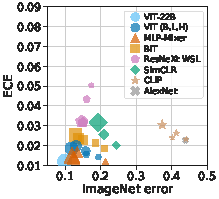
\includegraphics[width=0.35\textwidth]{figs/calibration_plex/vit22b_temperature_scaling_ts_no_title.pdf}}
    \caption{\chonk (light-blue circle) improves the Pareto frontier of the accuracy vs.~the calibration (ECE). Left/right panels are without/with temperature scaling, respectively.}
    \label{fig:calibration}
% \vspace{-10pt}
\end{figure}


\subsubsection{Distillation}
We perform model distillation~\citep{hinton2015distilling} to compress the \chonk into smaller, more widely usable ViTs.
We distill \chonk into ViT-B/16 and ViT-L/16 by following the procedure of~\citet{beyer2022knowledge}.
Using ImageNet-finetuned (at 384px) \chonk, we annotated 500 random augmentations and mixup transforms of each ImageNet image with \chonk logits.
Then, we minimize the KL divergence between the student and the teacher predictive distributions.
We train for 1000 epochs after initializing the student architecture from checkpoints pre-trained on JFT.
The results are shown in \cref{tab:distillation_imagenet}, and we see that we achieve new SOTA on both the ViT-B and ViT-L sizes.
% Appendix \todo{XYZ} contains further details.

\begin{table}[tbp]
%\vspace{-5pt}
    \caption{
      %\textbf
      Distillation results, finetuned at 384 resolution.
}
\centering
  \setlength{\tabcolsep}{4pt}
  \resizebox{0.6\textwidth}{!}{%
    \begin{tabular}{@{} l l c @{}}
      \toprule
	    Model      & &
	    ImageNet1k %Test 
	    \\
      \midrule
      \multirow[c]{4}{*}{\rotatebox{90}{ViT-B/16}}
    %   ViT-B/16~\citep{touvron2022deit} (scratch) & 85.0 \\
    %   ViT-B/16 distilled from \chonk (scratch) & \textbf{?} \\      
      %ViT-B/16
      &~\citep{dosovitskiy2020image} (JFT ckpt.) & 84.2 \\
      %ViT-B/16
      &~\citep{zhai2022scaling} (JFT ckpt.) & 86.6 \\
      %ViT-B/16
      &~\citep{touvron2022deit} (INet21k ckpt.) & 86.7 \\
      %ViT-B/16
      & Distilled from \chonk (JFT ckpt.) & \textbf{88.6} \\
      \midrule
    %   ViT-L/16~\citep{touvron2022deit} (scratch) & 85.8 \\
    %   ViT-L/16 distilled from \chonk (scratch) & \textbf{?} \\   
          \multirow[c]{4}{*}{\rotatebox{90}{ViT-L/16}}
      %ViT-L/16 
      &~\citep{dosovitskiy2020image} (JFT ckpt.) & 87.1 \\
      %ViT-L/16 
      &~\citep{zhai2022scaling} (JFT ckpt.) & 88.5 \\
      %ViT-L/16 
      &~\citep{touvron2022deit} (INet21k ckpt.) & 87.7 \\
      %ViT-L/16 
      & Distilled from \chonk (JFT ckpt.) & \textbf{89.6} \\ 
      \bottomrule
 \end{tabular}
 }
    \label{tab:distillation_imagenet}
    % \vspace{-10pt}
\end{table}
